% Options for packages loaded elsewhere
\PassOptionsToPackage{unicode}{hyperref}
\PassOptionsToPackage{hyphens}{url}
%
\documentclass[
]{article}
\usepackage{amsmath,amssymb}
\usepackage{iftex}
\ifPDFTeX
  \usepackage[T1]{fontenc}
  \usepackage[utf8]{inputenc}
  \usepackage{textcomp} % provide euro and other symbols
\else % if luatex or xetex
  \usepackage{unicode-math} % this also loads fontspec
  \defaultfontfeatures{Scale=MatchLowercase}
  \defaultfontfeatures[\rmfamily]{Ligatures=TeX,Scale=1}
\fi
\usepackage{lmodern}
\ifPDFTeX\else
  % xetex/luatex font selection
\fi
% Use upquote if available, for straight quotes in verbatim environments
\IfFileExists{upquote.sty}{\usepackage{upquote}}{}
\IfFileExists{microtype.sty}{% use microtype if available
  \usepackage[]{microtype}
  \UseMicrotypeSet[protrusion]{basicmath} % disable protrusion for tt fonts
}{}
\makeatletter
\@ifundefined{KOMAClassName}{% if non-KOMA class
  \IfFileExists{parskip.sty}{%
    \usepackage{parskip}
  }{% else
    \setlength{\parindent}{0pt}
    \setlength{\parskip}{6pt plus 2pt minus 1pt}}
}{% if KOMA class
  \KOMAoptions{parskip=half}}
\makeatother
\usepackage{xcolor}
\usepackage{graphicx}
\makeatletter
\def\maxwidth{\ifdim\Gin@nat@width>\linewidth\linewidth\else\Gin@nat@width\fi}
\def\maxheight{\ifdim\Gin@nat@height>\textheight\textheight\else\Gin@nat@height\fi}
\makeatother
% Scale images if necessary, so that they will not overflow the page
% margins by default, and it is still possible to overwrite the defaults
% using explicit options in \includegraphics[width, height, ...]{}
\setkeys{Gin}{width=\maxwidth,height=\maxheight,keepaspectratio}
% Set default figure placement to htbp
\makeatletter
\def\fps@figure{htbp}
\makeatother
\setlength{\emergencystretch}{3em} % prevent overfull lines
\providecommand{\tightlist}{%
  \setlength{\itemsep}{0pt}\setlength{\parskip}{0pt}}
\setcounter{secnumdepth}{-\maxdimen} % remove section numbering
\ifLuaTeX
  \usepackage{selnolig}  % disable illegal ligatures
\fi
\IfFileExists{bookmark.sty}{\usepackage{bookmark}}{\usepackage{hyperref}}
\IfFileExists{xurl.sty}{\usepackage{xurl}}{} % add URL line breaks if available
\urlstyle{same}
\hypersetup{
  pdftitle={Master APVV},
  hidelinks,
  pdfcreator={LaTeX via pandoc}}

\title{Master APVV}
\author{}
\date{}

\begin{document}
\maketitle

PAS BESOIN DE TOEIC OU AUTRE POUR RENTRER!!!!

Sont en dialogue avec les équipes info pour poster les infos sur
internet mais ils sont débordés.

La mention c\textquotesingle est \textbf{Biologie agrosciences} qui
regroupe à la fois du végétal et de l\textquotesingle animal (2
parcours, APVV et SAED).\\
Ils ont choisi cette mention pour s\textquotesingle adosser à
l\textquotesingle institut agro de rennes pcq il pensent que
c\textquotesingle est bénef pour tlm -\textgreater{} mutualisation :
échanges culturels entres fac et ingés

Mention biologie agroscience dirigée (co accrédité) : Joceline Flamand
(bio animale, agronomie, Institut agro) et Alain Bouchereau (bio
végétale, Université).

Parcours APVV
(\url{https://formations.univ-rennes.fr/master-mention-biologie-agrosciences-parcours-adaptation-protection-valorisation-du-vegetal-apvv})\\
Mélanie Jubault (généticienne quantitative, institu agro) et Antoine
Gravot (fac) coordonnent ce parcours au niveau scientifique et
administratif.

4 Mineures proposées

Historiquement le parcours était orienté sur le végétal mais partait
dans différentes directions, y avait notamment la dimension génétique
(amélioration), physio, agro, substances naturelles et améliorations.\\
La nouvelle version du master est centrée sur ce qu\textquotesingle on
peut apporter par rapport aux questions de transitions
agroécologiques.\\
On forme donc des cadres scientifiques qui ont besoin
d\textquotesingle une vision large sur tous les niveaux
d\textquotesingle approche (écologique/agronomie au niveau des systèmes,
génétique dans l\textquotesingle optique agroéco (conservation,
domestication, protection), physiologique (intéractions écologiques
notamment; on a décidé de mettre un accent fort sur la physiologie
\textbf{chimique}))\\
Vision interdisciplinaire mais pas l\textquotesingle impression que ces
disciplines soient juxtaposées.\\
Jusqu\textquotesingle à présent même chez les chercheurs
c\textquotesingle était assez cloisonné.\\
C\textquotesingle est comme ca qu\textquotesingle est basé le système de
majeures.

4 domaines sur lesquelles ils veulent focus (\textasciitilde mineures)
mais seront tous un minimum présentés dans le tronc commun.

\begin{enumerate}
\tightlist
\item
  en génétique, génomique et amélioration des plantes,
\item
  en physiologie de la plante et de ses adaptations aux stress,
\item
  en écologie des interactions plantes/bioagresseurs
\item
  sur le fonctionnement et la gestion des agrosystèmes.
\end{enumerate}

Compétences développées: on va rentrer dans des métiers ou les
connaissances vont évoluer vite, donc on attendra de nous
professionnellement d\textquotesingle être capable
d\textquotesingle évoluer, de s\textquotesingle adapter.\\
Donc surtout on va apprendre à identifier un probleme,
l\textquotesingle analyser, voir des solutions,
intégrer/s\textquotesingle adapter aux nouvelles connaissances.\\
\emph{pour plus de détails aller voir la description détaillée sur le
site}

Les plus de la formation : la co-accréditation bénéfique pour tout le
monde, regards différents, et aussi que tous les enseignants sont liés à
des instituts (inrae, cnrs, instituts techniques ou scientifiques) qui
permettent de faire venir des intervenants et ouvre des portes de stages
et de potentielles visites.

Poursuite d\textquotesingle études:

\begin{itemize}
\tightlist
\item
  partie relativement importante d\textquotesingle étudiants qui partent
  en thèse (peut se faire dans le public et dans des partenariats avec
  le privé (CIFRE)).\\
  \emph{pb des thèses est la dimension mobilité : on voit du pays
  (différents pays littéralement)}\\
  \emph{dans le cadre des thèses cifre c\textquotesingle est moins le
  cas}
\end{itemize}

\hypertarget{organisation-puxe9dagogique}{%
\subsubsection{Organisation
pédagogique:}\label{organisation-puxe9dagogique}}

\emph{programme détaillé en bas du site, pas encore update (falloir
attendre qq semaines -\textgreater{} tt est inclus (à jour) dans
organisation pédagogique}\\
Tronc commun avec le minimum à savoir sur tous les thèmes.

\hypertarget{les-ue-obligatoires-du-s1}{%
\subparagraph{Les ue obligatoires du
S1}\label{les-ue-obligatoires-du-s1}}

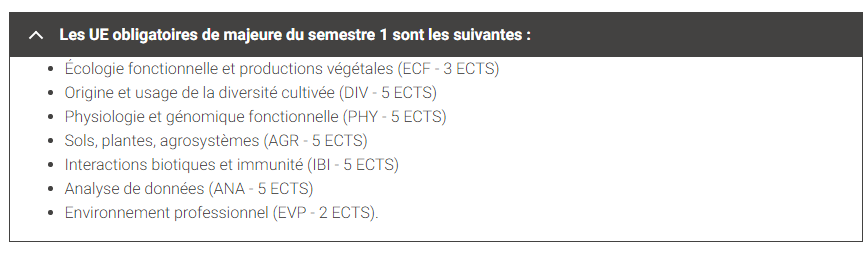
\includegraphics{./tex2pdf.-c51dec89c2ee7bdf/5f4acb47ce35eb7a88155dee39fad8e93d57bda7.png}\\
\textbf{UE interdisciplinaires}

\begin{itemize}
\tightlist
\item
  Ecologie fonctionnelle : introduction des différentes échelles et leur
  importance (sandrine monie (jsp l\textquotesingle orthographe), fac ;
  édith lecadre, institut agro)
\item
  Origine (armel salmon, paul simion (fac)) et usages (maria
  manzannares, Mélanie Jubault,... (institut agro)) de la diversité
  cultivée.
\item
  Physiologie (gravot, articulation avec des enjeux concrets, par
  exemple l\textquotesingle assimilation de l\textquotesingle azote) et
  génomique fonctionnelle
\item
  Sols, plantes et agrosystèmes (que des gens de
  l\textquotesingle institut agro) : panorama global destiné à tout le
  monde
\item
  Interactions biotiques et immunité (christophe lemai et florence val,
  profs à l\textquotesingle agro, et edith lecadre) : bioagresseurs,
  symbioses, comment ca s\textquotesingle articule avec des pratiques
  professionnelles.
\end{itemize}

UE transversales

\begin{itemize}
\tightlist
\item
  Analyses de données : in peu d\textquotesingle informatique (comment
  gérer des gros tableaux de données), des statistiques (gros pole de
  stat à l\textquotesingle institut agro, références nationales).
\item
  Environnement professionnel
\end{itemize}

\hypertarget{les-ue-du-s2}{%
\subparagraph{Les ue du S2}\label{les-ue-du-s2}}

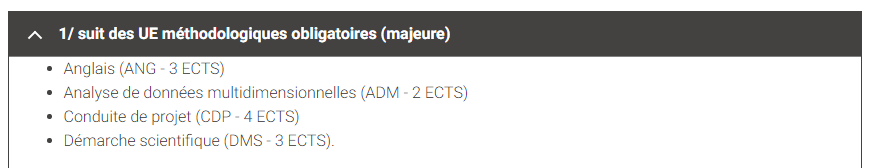
\includegraphics{./tex2pdf.-c51dec89c2ee7bdf/768f3bd7e1263dcf1a33d1386e976f4a4a68ff28.png}

\begin{itemize}
\tightlist
\item
  Anglais (sur tout l\textquotesingle année en vrai)
\item
  Analyses de données multidimensionnelles (suite des stats)
\item
  Démarche scientifique : on vérifié qu\textquotesingle on sait faire de
  la synthèse biblio, qui peut correspondre au stage effectué durant le
  S2 (permet de préparer le stade), ou peut être articulé avec la
  conduite de projet
\item
  conduite de projet, à l\textquotesingle inra du Reu, sur 1 semaine (en
  un coup ou 1j/semaine), on nous pose une question, on fait la biblio,
  on co-construit l\textquotesingle experimentation, chaque spé/type de
  centre d\textquotesingle intérêt vont analyser une partie des
  résultats (même si on touche à tout), permettra
  d\textquotesingle utiliser aussi les trucs vus en stat
\end{itemize}

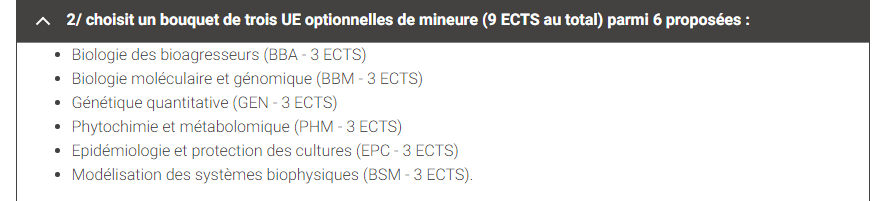
\includegraphics{./tex2pdf.-c51dec89c2ee7bdf/010a3db66a1b14f8f965e3622e83d80b73e1a10a.png}\\
L\textquotesingle objectif est de choisir exactement ce
qu\textquotesingle on veut en ue parce que l\textquotesingle idée
c\textquotesingle est que tt les disciplines vont potentiellement
contribuer à la transition et on sait pas quelle association de
disciplines va être la plus importante dans le futur.\\
Ceci étant dit, selon la mineure désirée en M2, on peut en avoir des
"fortement recommandée/obligatoires"

\begin{itemize}
\tightlist
\item
  GEN : pour apprendre à faire des QTL (quantitative trait loci),
  analyse génétique
\item
  BBM : techniques de séquencage, transgénèse, etc
\item
  BBA : traité par l\textquotesingle Institut : y a bcp de
  bioagresseurs, faut connaitre leur fonctionnement, leur cycle et site
  de vie, que ce soit champis, insectes, etc.... c\textquotesingle est
  en lien avec la pratique et les pbs actuels.
\item
  PHM : connaissances et méthodo moderne pour analyser la chimie associé
  à des processus biologiques, domaine hyper en développement
  actuellement, s\textquotesingle adresse aux gens qui
  s\textquotesingle intéressent à la physio, mais aussi à
  l\textquotesingle écologie des intéractions,
  s\textquotesingle intéressent aussi aux polluants.
\item
  EPC : méthodes mathématiques et pratiques et comment
  l\textquotesingle appliquer à la protection
\item
  BSM : questions relative à l\textquotesingle eau et sa modélisation
  dans les agrosystèmes et paysages : modélisation mathématique.
\end{itemize}


\includegraphics{./tex2pdf.-c51dec89c2ee7bdf/3dc69885aa24c13a453708449cc1311651841e1e.png}\\
Soutenance fin juin

\hypertarget{les-ues-du-s5}{%
\subparagraph{Les ues du S5}\label{les-ues-du-s5}}

Tronc commun\\
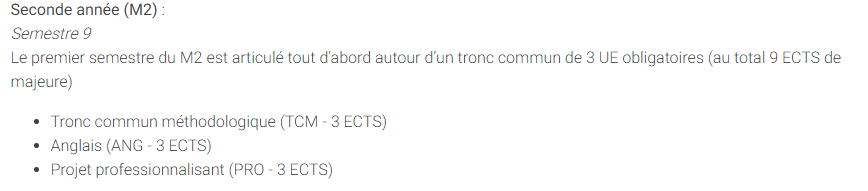
\includegraphics{./tex2pdf.-c51dec89c2ee7bdf/4b78bfee45bbe365c9ba664b8d937d784044e007.png}

\begin{itemize}
\tightlist
\item
  projet professionnalisant varie selon les mineures choisies.
\end{itemize}

4 mineures ( ya des ues potentiellement mutualisées)

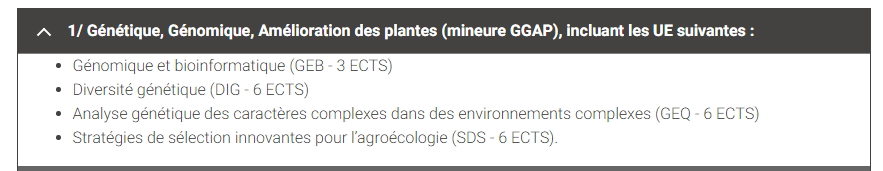
\includegraphics{./tex2pdf.-c51dec89c2ee7bdf/38e89372575bd20755ba85048463dd0190fe5060.png}

\begin{itemize}
\tightlist
\item
  GEB : méthodo essentiellement des outils informatiques
\item
  DIG :
\item
  GEQ : analyses QTL, pas mal de maths/stats
\item
  SDS : comment utiliser les autres ues pour sélectionner bien,
  dialoguer avec les autres disciplines,...\\
  Formation connue en France, y a ici, montpellier, et 3 étudiants cette
  années à agroparis\\
  Le métier de sélectionneur n\textquotesingle est pas du bureau,
  c\textquotesingle est bcp de terrain et d\textquotesingle observation
  des plantes
\end{itemize}

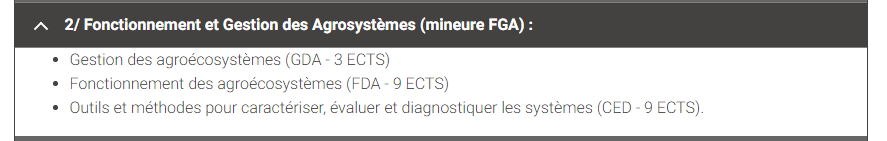
\includegraphics{./tex2pdf.-c51dec89c2ee7bdf/65bd4328028286600d01f432b822ae8897ae5b25.png}\\
Une ue après l\textquotesingle autre dans l\textquotesingle edt, on veut
nous apprendre à caractériser les différentes organisations, itinéraires
techniques.\\
Montrent des outils qui permettent de rigoureusement comparer els
différentes organisations d\textquotesingle agrosystèmes, et être
capable de diagnostiquer un dispositif, et proposer des améliorations
possibles.\\
Formation reconnue, orientée vers la production.

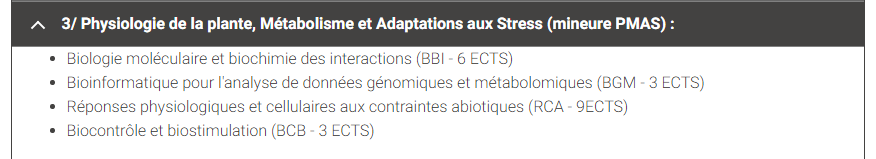
\includegraphics{./tex2pdf.-c51dec89c2ee7bdf/71db356ee1167ee29b643ab54cb9525fdd404eeb.png}\\
gravot en est responsable

\begin{itemize}
\tightlist
\item
  BBI : interactions plantes bioagresseurs et plantes microorganismes
  bénéfiques....
\item
  BGM : analyse du métabolome
\item
  RCA : l\textquotesingle équivalent de la première mais en abiotique
\item
  BCB : comment peut ont utiliser les notions précédentes pour controler
\end{itemize}

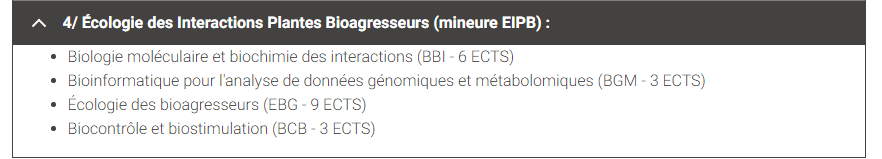
\includegraphics{./tex2pdf.-c51dec89c2ee7bdf/7e798685fc885fd4d6ae9a80647c5a4db1dfcebc.png}\\
Relativement soeur de la mineure PMAS (3 UE/4 partagées)\\
L\textquotesingle ue qui change : EBG\\
Dimension en écologie bcp plus forte.

Fin du master en juin (plus tot que d\textquotesingle autres) : pcq 20
\% des gens se destinent à la thèse donc faut déjà avoir le diplome pcq
bourses de thèse (suis pas sur d\textquotesingle avoir bien entendu)
données fin juin

Modalité de controle des connaissances : controle continu intégral au
M1, et mélange de controle continu et des partiels au M2 (ex: FGA, grand
oral très long ou on remobilise l\textquotesingle ensembnle des cours
\textbar{} en physio il y a dissertation de 4h, avec cours et documents
autorisés )

Responsables pédagogiques : contacts en bas de la page du site

\end{document}
